\section{متحكم تناسبي-تكاملي-تفاضلي (\LR{PID Control})}
\label{sec:pid_control}

\subsection*{1. مبدأ الخوارزمية}
يُعد متحكم (\LR{PID}) خوارزمية تحكم خطية كلاسيكية تعتمد على الاستقلالية؛ حيث تعامل كل مفصل كنظام مستقل تماماً، وتتعامل مع التداخلات الديناميكية بين المفاصل وتغيرات الكتلة على أنها مجرد اضطرابات خارجية دون الحاجة لمعرفة النموذج الرياضي للنظام.

\subsection*{2. الشكل العام لقانون التحكم}
يُعطى قانون التحكم الكلاسيكي المستقل لكل مفصل بالصيغة الرياضية القياسية التالية:
\begin{equation}
u(t) = K_p e(t) + K_i \int_{0}^{t} e(\tau) d\tau + K_d \dot{e}(t)
\end{equation}
حيث $K_p, K_i, K_d$ تمثل أرباح التناسب، التكامل، والتفاضل على التوالي.

\subsection*{3. تهيئة النموذج وتعريف الأخطاء}
باعتبار الشعاع $q_{ref}$ يمثل المسار المرجعي المطلوب، والشعاع $q$ يمثل الموضع الفعلي للمفصل، يتم تعريف شعاع خطأ التتبع الموضعي $e$ وشعاع خطأ السرعة $\dot{e}$ لمفاصل الروبوت الثلاثة كما يلي:
\begin{equation}
e = \begin{bmatrix} \theta_{1ref} - \theta_1 \\ \theta_{2ref} - \theta_2 \\ d_{3ref} - d_3 \end{bmatrix} , \quad 
\dot{e} = \begin{bmatrix} \dot{\theta}_{1ref} - \dot{\theta}_1 \\ \dot{\theta}_{2ref} - \dot{\theta}_2 \\ \dot{d}_{3ref} - \dot{d}_3 \end{bmatrix}
\end{equation}

\subsection*{4. تطبيق الخوارزمية على النموذج}
يُصاغ شعاع إشارة التحكم الكلية $U_{PID}$ لجميع المفاصل بالشكل المصفوفي:
\begin{equation}
U_{PID} = K_P e + K_I \int e dt + K_D \dot{e}
\end{equation}
حيث $K_P, K_I, K_D$ هي مصفوفات قطرية تحوي أرباح التحكم لكل مفصل. بتعويض إشارة التحكم في النموذج الديناميكي الشامل للروبوت المستنتج في الفصل السابق، تصبح معادلة النظام المغلق:
\begin{equation}
\ddot{q} = \bar{M}^{-1} \left[ A \left( K_P e + K_I \int e dt + K_D \dot{e} \right) - R \dot{q} - D \right]
\end{equation}
\subsection{5. استجابة النظام عند قيم مختلفة للحمل ($m_L$)}
تم اختبار خوارزمية (\LR{PID}) عبر محاكاة تتبع إشارات مرجعية خطية (\LR{Step Response}) للمفاصل الثلاثة، حُددت بالقيم التالية: $\theta_{1ref} = 90^\circ$، $\theta_{2ref} = 90^\circ$، و $d_{3ref} = 0.2 \text{ m}$. يوضح الشكلان التاليان استجابة المفاصل عند تطبيق الخوارزمية باختبارين مختلفين لكتلة الحمل المرفوع ($m_L$):

\begin{figure}[H]
    \centering
    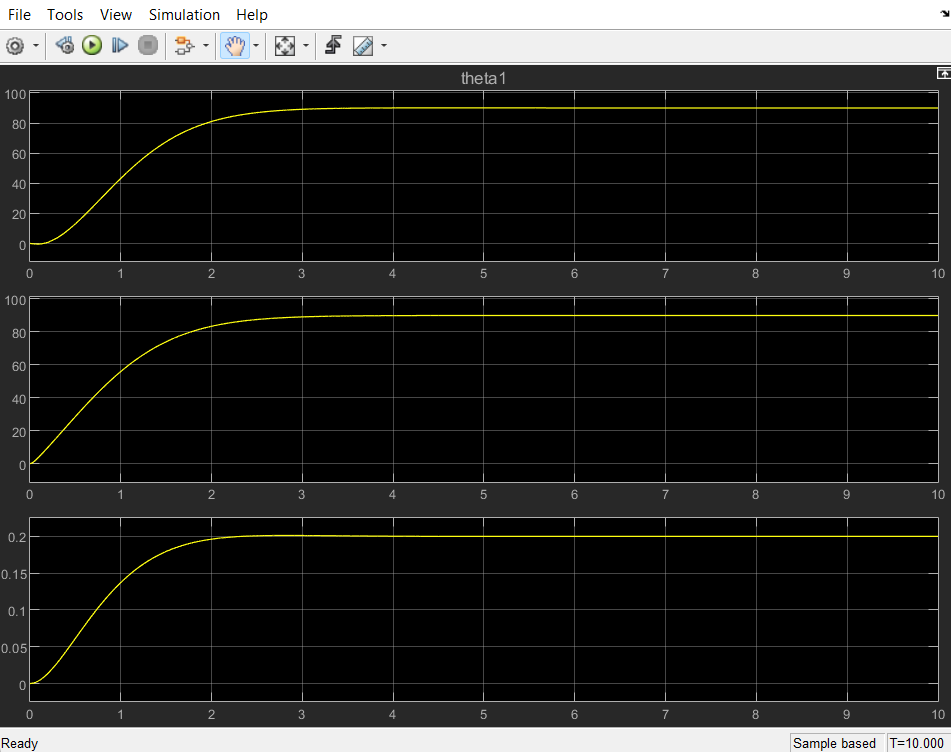
\includegraphics[width=0.8\textwidth]{resources/images/PID_res_m0.png}
    \caption{\centering{استجابة متحكم \LR{PID} بدون حمل ($m_L = 0 \text{ kg}$)}}
    \label{fig:pid_m0}
\end{figure}
  

\begin{figure}[H]
    \centering
    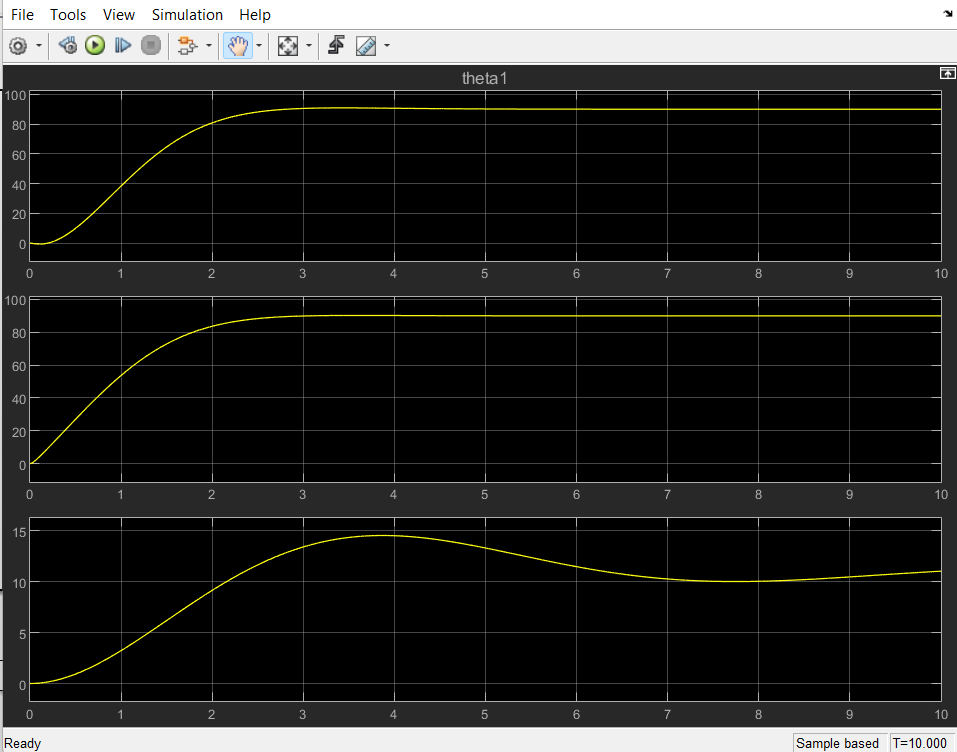
\includegraphics[width=0.8\textwidth]{resources/images/PID_res_m10.png}
    \caption{\centering{استجابة متحكم \LR{PID} عند إضافة حمل ($m_L = 10 \text{ kg}$)}}
    \label{fig:pid_m10}
\end{figure}

يُلاحظ من الشكل (\ref{fig:pid_m0}) أن المتحكم في حالة اللاحمل ($m_L = 0$) قادر على توجيه المفاصل نحو القيم المرجعية بدقة واستقرار تام وبدون خطأ حالة مستقرة. 

في المقابل، عند إضافة حمل كتلته ($10 \text{ kg}$) كما في الشكل (\ref{fig:pid_m10})، يتدهور أداء المتحكم الكلاسيكي بشكل حاد. يظهر هذا الانهيار بوضوح شديد في المفصل الانسحابي ($d_3$)، حيث ينحرف المسار الفعلي بشكل كارثي مبتعداً عن القيمة المرجعية ($0.2$) ليصل إلى قيم تفوق ($14$). يعود هذا الفشل إلى عجز أرباح الـ (\LR{PID}) الثابتة عن توليد إشارة تحكم كافية لتعويض الزيادة الضخمة في قوى الجاذبية وعزوم القصور الذاتي الناتجة عن الحمل الجديد، مما يثبت افتقار هذه الخوارزمية للمتانة (\LR{Robustness}) المطلوبة في التطبيقات الصناعية متغيرة الأوزان.